\documentclass{cubeamer}

\title{Zjawisko fotoelektryczne}
\subtitle{Programy użytkowe}
\author[Natalia S. \and Tomasz T. \and Kacper M.]{Natalia Serwin \and Tomasz Targiel \and Kacper Mordarski}
\date{Styczeń 2021}
\institute[Uniwersytet Wrocławski]{Fizyka komputerowa, Wydział Fizyki i Astronomii, Uniwersytet Wrocławski}

\begin{document}
	\maketitle

	\cutoc

	\section{Fotony}

	\begin{frame}{Odrobina historii}
		\begin{columns}
			\begin{column}{0.4\textwidth}
				\begin{figure}
					\centering
					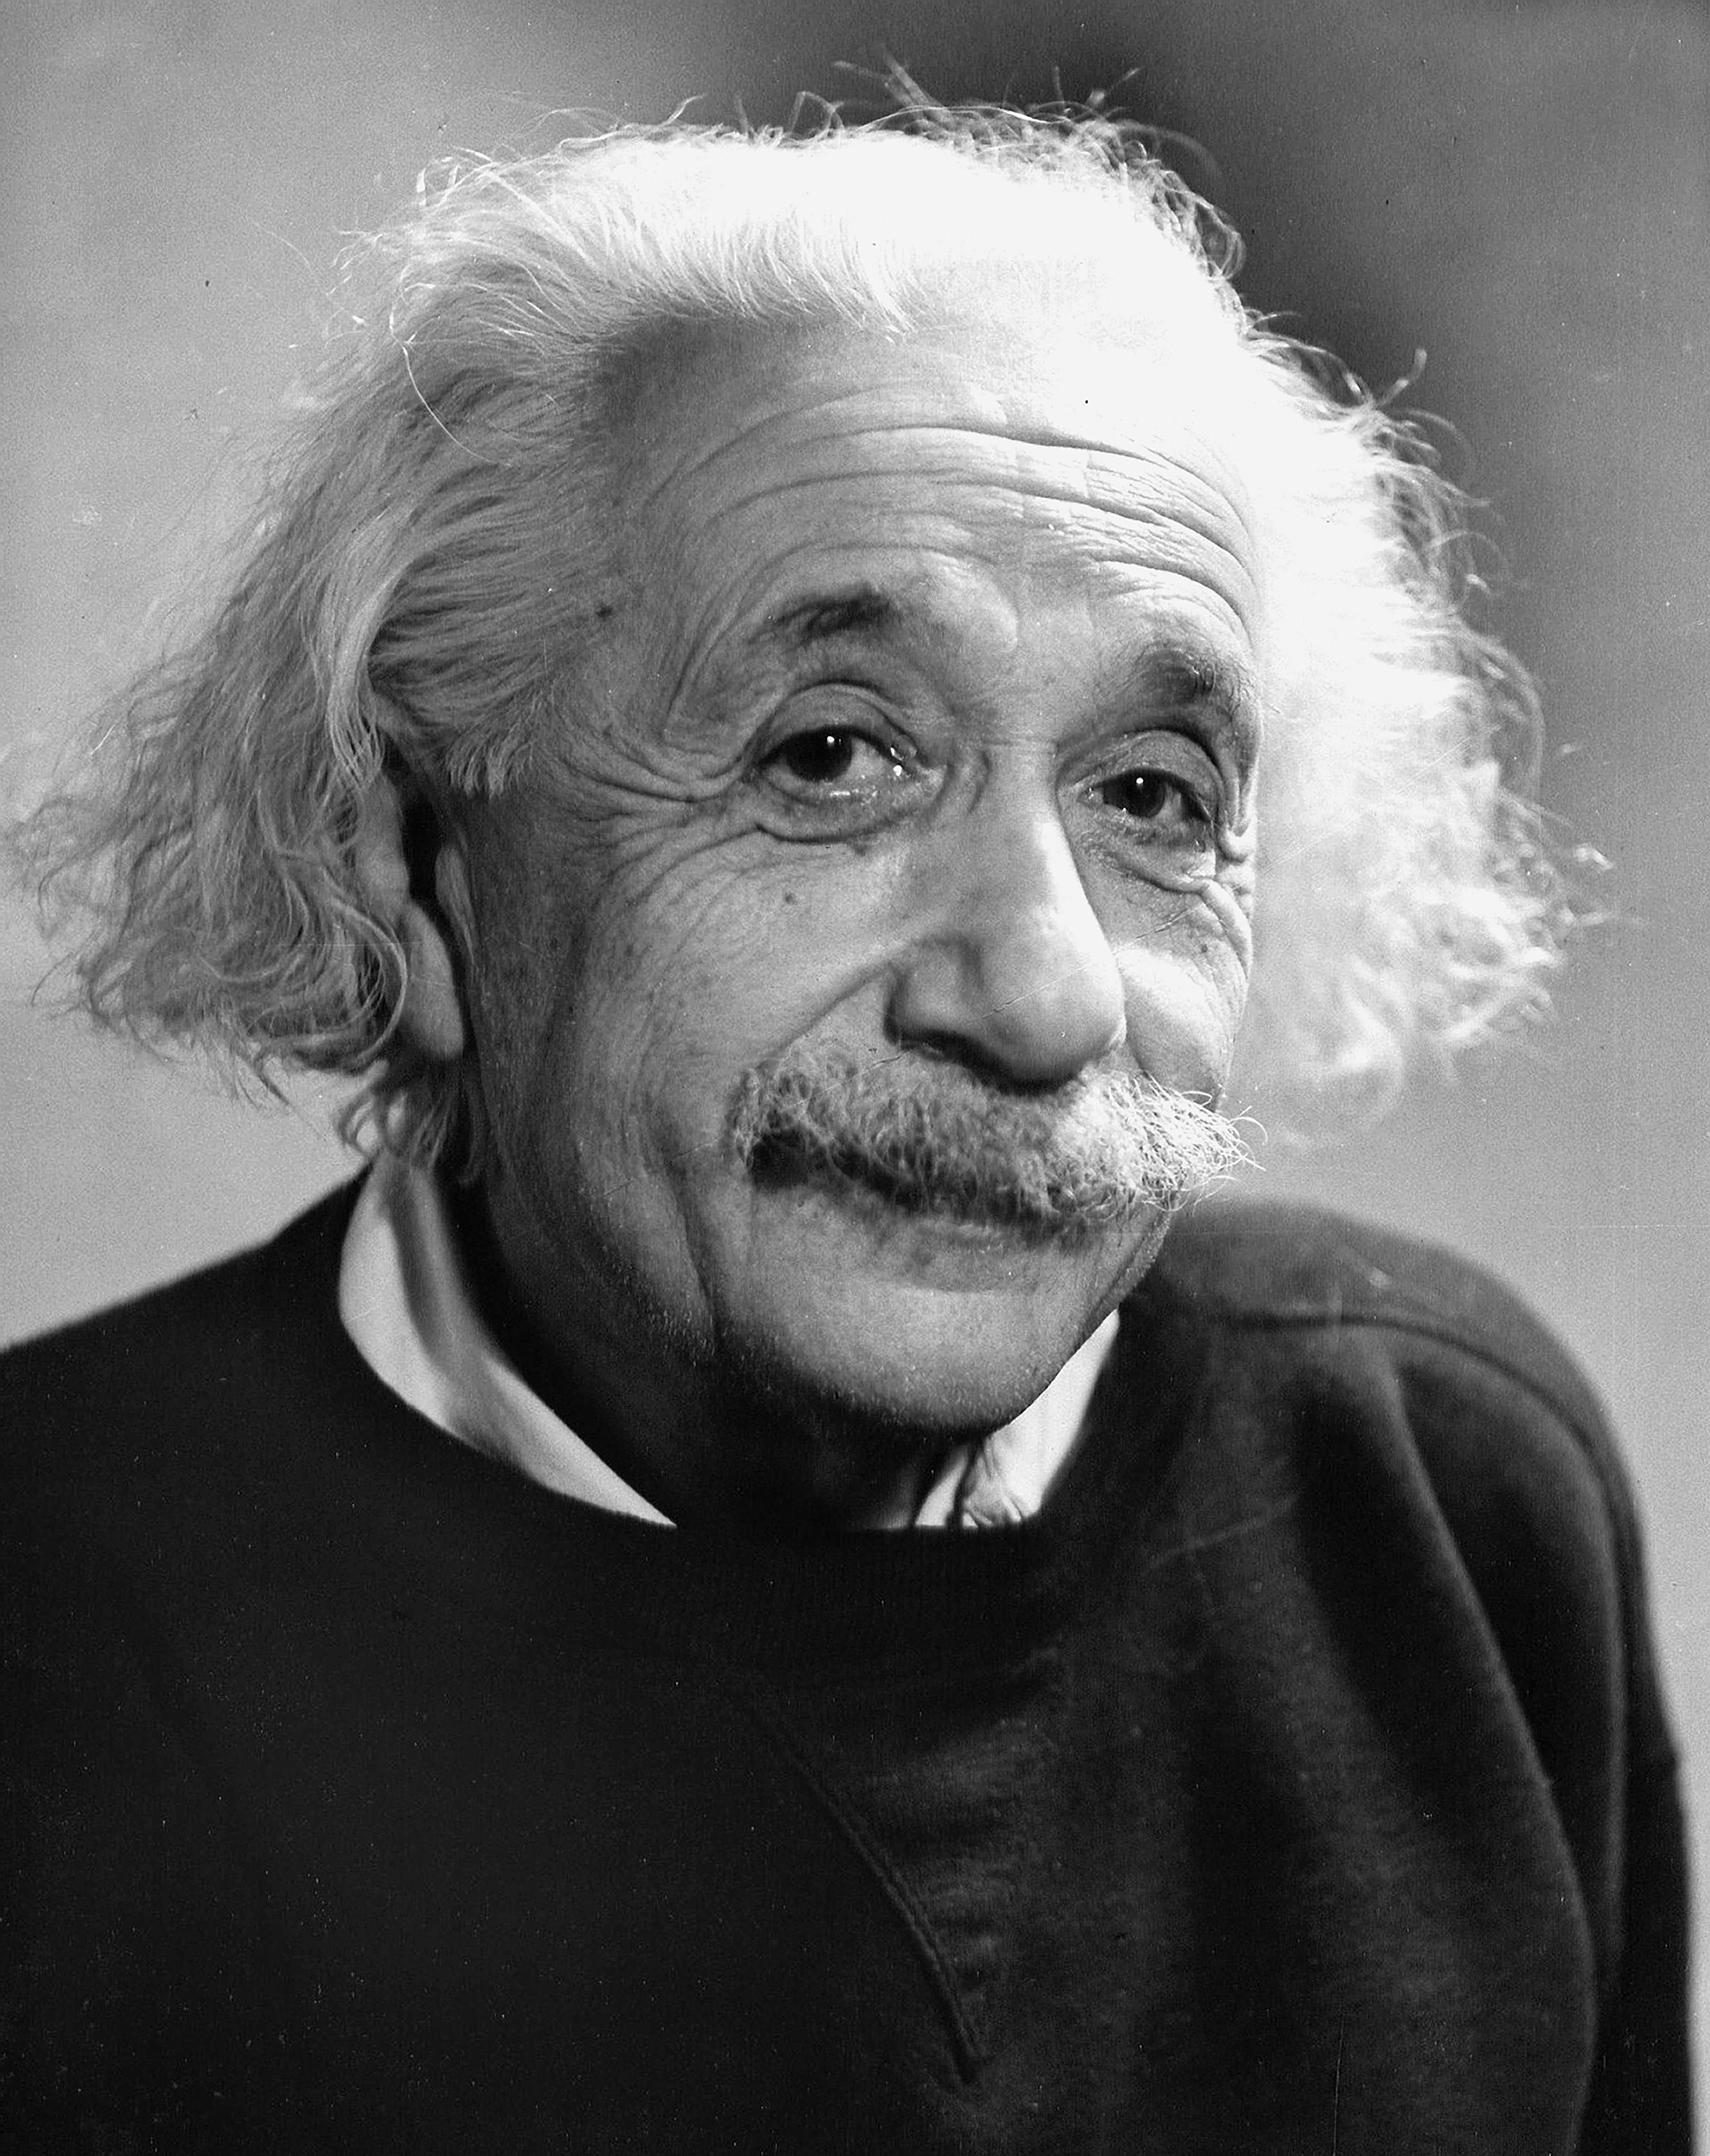
\includegraphics[height=0.7\textheight]{img/albert.jpeg}
					\caption{Albert Einstein}
				\end{figure}
			\end{column}
			\begin{column}{0.6\textwidth}
				Albert Einstein wykazał, że światło nie tylko jest emitowane porcjami, ale
				rozchodzi się w przestrzeni jako zbiór cząstek – fotonów – i jest pochłaniane
				również porcjami.
				\newline
				\newline
				Było to niezwykłe odkrycie, gdyż do tej pory uważano, że światło to fala
				elektromagnetyczna, a wszystkie zjawiska optyczne doskonale wyjaśniała falowa
				teoria światła.
			\end{column}
		\end{columns}
	\end{frame}

	\begin{frame}{Doświadczalne przedstawienie zjawiska fotoelektrycznego}
		\begin{columns}
			\begin{column}{0.5\textwidth}
				W szklanej bańce, w której panuje wysoka próżnia, znajdują się dwie metalowe
				elektrody A i B. Światło pada na metalową płytkę A i uwalnia z niej
				elektrony, które nazywamy fotoelektronami.
				\newline
				\newline
				Fotoelektrony są rejestrowane jako prąd elektryczny płynący między
				płytką A oraz elektrodą zbierającą B przy przyłożonym napięciu U.
			\end{column}
			\begin{column}{0.5\textwidth}
				\begin{figure}
					\centering
					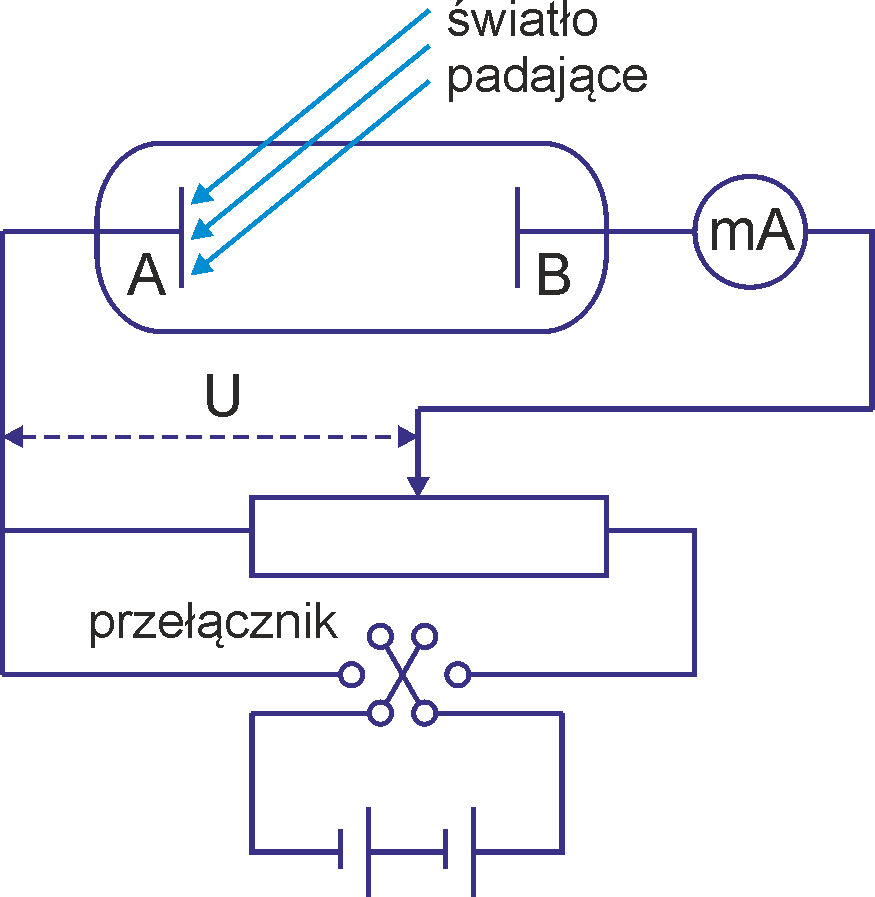
\includegraphics[height=0.6\textheight]{img/rysunek_1.1.png}
					\caption{Schemat układu doświadczalnego do badania tego zjawiska}
				\end{figure}
			\end{column}
		\end{columns}
	\end{frame}

	\section{Cechy efektu fotoelektrycznego}

	\begin{frame}{Brak opóźnienia}
		Gdy promieniowanie pada na metalową płytkę elektrody, elektrony emitowane są
		natychmiast, nawet przy bardzo niewielkim natężeniu promieniowania. Brak
		opóźnienia stoi w sprzeczności z fizyką klasyczną, w ramach której przewiduje
		się, że zwłaszcza przy niskim natężeniu padającego światła powinno minąć
		nieco czasu, zanim elektrony pobiorą wystarczającą ilość energii, aby
		uwolnić się z powierzchni metalu. Takie opóźnienie nie jest jednak obserwowane.
	\end{frame}

	\begin{frame}{Natężenie padającego promieniowania, a energia kinetyczna elektronów}
		\begin{columns}
			\begin{column}{0.5\textwidth}
				\begin{figure}
					\centering
					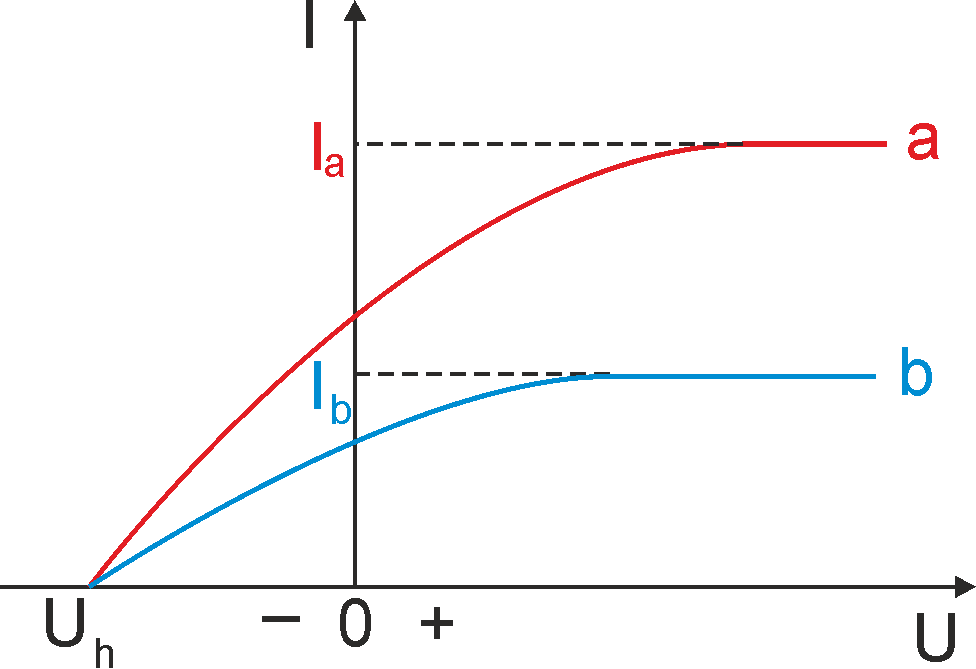
\includegraphics[height=0.5\textheight]{img/rysunek_1.2.png}
					\caption{Zależność prądu fotoelektrycznego od przyłożonego napięcia U}
				\end{figure}
			\end{column}
			\begin{column}{0.6\textwidth}
				Opuszczający powierzchnię płytki fotoelektron ma energię kinetyczną $E_{k0}$,
				którą uzyskał od padającego promieniowania. Jego energia potencjalna zmienia
				się o $q\Delta V$, gdzie $\Delta V$ jest różnicą potencjałów, a q=-e.

				Z zasady zachowania energii wynika więc, że $\Delta E_{k}-e\Delta V=0J$ ($\Delta
				E_{k}$
				-zmiana energii kinetyczej fotoelektronu). Gdy przyłożymy napięcie hamowania
				$-\Delta V_{h}$ , fotoelektron traci całą swoją energię kinetyczną $E_{ki}$
				i zatrzymuje się.
			\end{column}
		\end{columns}
	\end{frame}

	\begin{frame}{Natężenie padającego promieniowania, a energia kinetyczna elektronów}
		\begin{columns}
			\begin{column}{0.5\textwidth}
				\begin{figure}
					\centering
					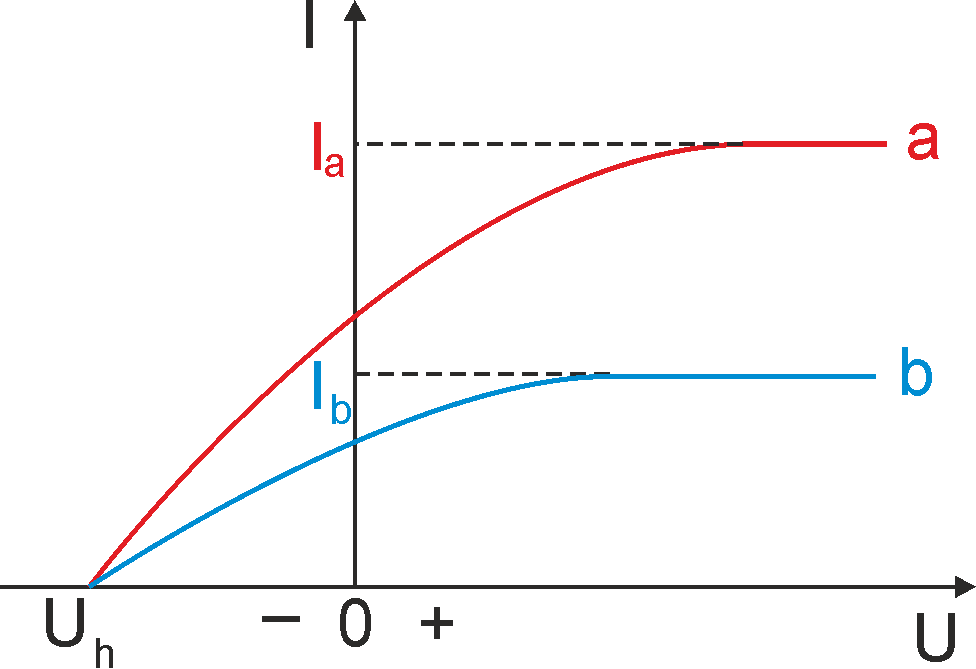
\includegraphics[height=0.5\textheight]{img/rysunek_1.2.png}
					\caption{Zależność prądu fotoelektrycznego od przyłożonego napięcia U}
				\end{figure}
			\end{column}
			\begin{column}{0.6\textwidth}
				Bilans energetyczny wyraża się wtedy następująco:
				$(0J-E_{k0})-e(-\Delta V_{h})=0J$, z czego wynika, że
				$E_{k0}=e\Delta V_{h}$. Napięcie hamowania pozwala nam więc wyznaczyć maksymalną
				energie kinetyczną $E_{kmax}$ emitowanych elektronów
				\begin{equation*}
					E_{kmax}=e\Delta V_{h}
				\end{equation*}
				Napięcie hamowania, a więc i maksymalna wartość energii kinetycznej
				fotoelektronów nie zależą od natężenia światła.
			\end{column}
		\end{columns}
	\end{frame}

	\begin{frame}{Częstotliwość progowa}
		Dla każdej metalowej powierzchni, na którą pada promieniowanie, istnieje pewna
		częstotliwość tego promieniowania, poniżej której nie rejestruje się
		fotoprądu – innymi słowy zjawisko fotoelektryczne nie zachodzi. Wielkość taką
		nazywamy częstotliwością progową i jest ona charakterystyczna dla danego metalu.

		Dane eksperymentalne pokazują liniową zależność – maksymalna energia kinetyczna
		fotoelektronów rośnie liniowo ze zwiększającą się częstotliwością padającego
		promieniowania.
	\end{frame}

	\begin{frame}{Częstotliwość progowa}
		\begin{columns}
			\begin{column}{0.5\textwidth}
				\begin{figure}
					\centering
					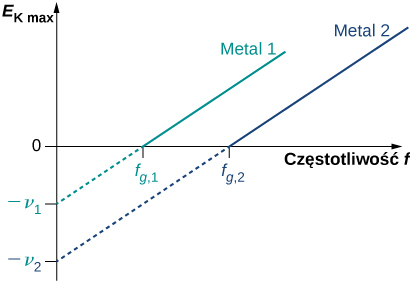
\includegraphics[height=0.4\textheight]{img/rysunek_1.3.jpeg}
					\caption{Liniowy wzrost energii kinetycznej ze zwiększającą się
					częstotliwością podającego promieniowania}
				\end{figure}
			\end{column}
			\begin{column}{0.6\textwidth}
				Pomiary dokonywane dla różnych metali dają liniową zależność z tym samym
				nachyleniem wykresu. Żadna z tych obserwacji nie daje się pogodzić z
				fizyką klasyczną(energia kinetyczna fotoelektronów powinna zależeć od
				natężenia padającego światła). Fizyka klasyczna nie przewiduje istnienia
				częstotliwości progowej. W klasycznym obrazie elektrony pobierają energię
				od promieniowania w sposób ciągły, ich energia kinetyczna powinna
				zależeć tylko od natężenia padającego światła, a efekt powinien zachodzić
				zawsze, niezależnie od częstotliwości.
			\end{column}
		\end{columns}
	\end{frame}

	\section{Kwantowa teoria Einsteina zjawiska fotoelektrycznego}

	\begin{frame}{Historia}
		Efekt fotoelektryczny został wyjaśniony w 1905 roku przez Alberta Einsteina.
		Założył on, że skoro hipoteza Plancka o kwantach energii poprawnie opisywała
		wymianę energii między promieniowaniem elektromagnetycznym i ścianami wnęki,
		to powinna być ona także zastosowana do opisu absorpcji promieniowania przez
		fotoelektrodę. Zapostulował on tezę, że fala elektromagnetyczna niesie
		energię w dyskretnych porcjach. Einstein rozszerzył hipotezę Plancka,
		postulując, że samo światło składa się z kwantów promieniowania (fotonów).
		Innymi słowy, że fale elektromagnetyczne są skwantowane.
	\end{frame}

	\begin{frame}{Energia pojedynczego fotonu}
		W podejściu Einsteina wiązka monochromatycznego światła o częstotliwości $\mathcal{V}$
		złożona jest z fotonów, czyli foton jest cząstką światła. Każdy foton porusza
		się z prędkością światła i niesie kwant energii $E_{f}$. Energia fotonów
		zależy tylko od częstotliwości $\mathcal{V}$ i dana jest wzorem:
		\begin{equation}
			E_{f}=h\mathcal{V}
		\end{equation}
		gdzie h jest stałą Plancka.
	\end{frame}

	\begin{frame}{Efekt fotoelektryczny}
		Jeżeli do wyrwania elektronu z metalu potrzebna jest energia $\mathcal{W}$,
		to wówczas:
		\begin{equation}
			h\mathcal{V}=\mathcal{W}+E_{kmax}
		\end{equation}
		Wielkość $\mathcal{W}$ charakterystyczna dla danego metalu nazywana jest pracą
		wyjścia.
		\newline
		\newline
		Zgodnie z powyższą zależnością energia $h\mathcal{V}$ fotonu, w części ($\mathcal{W}$)
		zostaje zużyta na wyrwanie elektronu z materiału (jego przejście przez
		powierzchnię), a ewentualny nadmiar energii ($h\mathcal{V}-\mathcal{W}$)
		elektron otrzymuje w postaci energii kinetycznej, przy czym część z niej może
		być stracona w zderzeniach wewnętrznych (przed opuszczeniem materiału).
	\end{frame}

	\begin{frame}[standout]
		\Huge\textsc{Dziękujemy za uwagę}

		\vfill

		\LARGE\textsc{Czy macie jakieś pytania?}
	\end{frame}
\end{document}